%  Robotics Text  by Jacob Rosen and Blake Hannaford
% (c) 2007  Jacob Rosen and Blake Hannaford
%

\chapter{Coordinate Transformations and Rigid Body Motions}

To properly control the manipulation of objects with robots, we must have precise and useful ways to describe their position and orientation.  In this chapter we start out with some definitions, and then develop the mathematical tools for this surprisingly non-straightforward task.   Finally we will combine position and orientation into a clever 4x4 matrix which represents both in one object.

%%%%** Section 1
\section{Problem Statement and Learning Objectives}
% Problem Statement and Learning Objectives for Chapter 02
\paragraph{Problem Statement}
 The problem this chapter addresses is to represent the position and orientation of rigid bodies and frames of reference in useful ways. 

\paragraph{Learning Objectives}
Upon completing this Chapter, the reader should be able to 
\begin{itemize}
	\item  Work with vectors and vector products.
	\item  Derive several mathematical represenations of 3D rigid body rotation
	\item  Represent any displacement and rotation of a rigid body by a 4x4 matrix (the homogeneous transformation).
        \item  Solve for unknown spatial relationships in terms of known spatial relationships using homogeneous transformations and transform graphs. 
\end{itemize}



%%%%** Section 2
\section{Description of Position and Orientation}

%%%%** Section 2.1
\subsection{Vectors and Translation}

We use vectors to represent the location of objects and also to represent translation movements from one point to another.


%
% \subsubsection{Unit Vector}
% \subsubsection{Difference between Vectors}
%%%%** Section 2.1.1
\subsubsection{Vector Cross Product}
We will sometimes need the vector cross product which is briefly defined here.

The cross product of two vectors, represented
\[
c = a \times b
\]
is a vector who's magnitude is
\[
|c| = |a||b|\sin(\theta)
\]
where $\theta$ is the angle between the two vectors.
and whos direction is orthogonal to both $a$ and $b$.  There are two orthogonal directions to $a$ and $b$ and the cross product sign is set by the right hand rule (sweeping the fingers from $a$ to $b$ and observing direction of thumb).   We will frequently consider the cross product of vectors separated by $90^\circ$ (for example the $X$ and $Y$ axes) and in this case
\[
|c| = |a||b|
\]

Another, equivalent, definition of the vector cross product can be expressed in matrix notation as
\[
a\times b = \left [
\begin{array}{ccc}
0 & -a_3 & a_2 \\
a_3 & 0 & -a_1 \\
-a_2 & a_1 & 0 \end{array} \right]
b
\]




\begin{ExampleSmall}
1) Find the magnitude of the cross product $a \times b$ where
\[
a = [ 3 \quad 4 \quad 7]^T \qquad \qquad  b = [ 2 \quad 4 \quad-3]^T
\]

\vspace{0.2in}

\[
c = a \times b
\]
\[
|c| = |a||b| = 8.6 \times 5.39 = 46.3
\]

2) Find the elements of the cross product.

\vspace{0.2in}
To get the components, it is easiest to use the matrix definition:
\[
c = \left [
\begin{array}{ccc}
0 & -7 & 4 \\
7 & 0 & -3 \\
-4 & 3 & 0 \end{array} \right]
\left [
\begin{array}{c}
2 \\ 4 \\ -3
\end{array}
\right ]        =
\left [
\begin{array}{c}
-40 \\ 23 \\ 4
\end{array}
\right ]
\]

You can verify that the magnitude of this vector is also 46.3.
\end{ExampleSmall}




%%%%** Section 2.2
\subsection{Coordinate Systems and Frames}

Of course when we use them numerically, our vectors must be defined with respect to axes in space.   Such a coordinate system contains three axes oriented to measure displacement in each of the three spatial dimensions.   We denote these axes $x,y,z$ and we will require that this system is {\it right handed} so that

\[
x \times y = z
\]
where $\times$ represents the vector cross product.
We can have as many coordinate systems as we like and they can differ from one another in two ways.  The location of their origin can be different, in which case we say they are {\it offset} or {\it displaced} from one another, and their orientation can be different, in which case we say they are {\it rotated} from one another.

 Another term for coordinate system is {\it reference frame} or simply {\it frame}.

%%%%** Section 2.3
\subsection{Points}
The numerical value or location of a point in space is only defined  with respect to a selected coordinate system.   Thus if we have a point, $P$, and a coordinate system, $A$, it will have a specific numerical location with respect to $A$. For example:
\[
^AP = \left [
\begin{array}{c}   1.7 \\ 0.25 \\ -3.1 \end{array}
\right ]
\]
While $P$ designates the point in the abstract, we add the leading subscript, $^AP$ to indicate $P$'s representation in coordinate system $A$.

The origin of a frame is also a point.   The displacement between two frames can thus be represented by a point, the origin of one frame, expressed in a second frame.   For example, imagine that  $M$ and $N$, are two coordinate systems not rotated with respect to each other, but their origins, $O_M$ and $O_N$, are separated by 5 cm in the x direction. Then
\[
^MO_N = [0.05  \quad 0.0 \quad 0.0]^T
\]
and
\[
^NO_M = [-.05 \quad 0.0 \quad 0.0]^T
\]




%%%%** Section 2.4
\subsection{Rigid Objects}
We will view rigid objects as a collection of points with a fixed relationship to one another.   How can we describe a rigid object's configuration in space with respect to some base frame, frame $B$?

%%%%** Figure 1
\begin{figure}
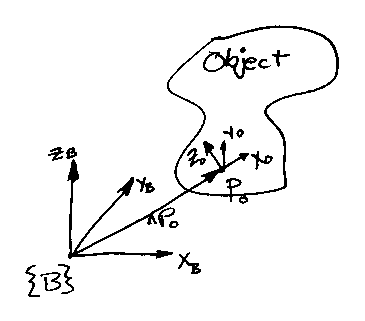
\includegraphics[width=3.5in]{figs02/00322.eps}
\caption{Representation of a rigid object in terms of an origin, $P_0$, and a frame attached to the object (frame $0$).}\label{ObjectLocationOrientation}
\end{figure}

First choose a point on the object, $P_0$ (Figure \ref{ObjectLocationOrientation}).    Then create a frame, $O$, whos origin is $P_0$.   The origin of $P_0$ does not have to be on or inside the object as long as all points in the object have a {\it fixed} representation in frame $O$.   The orientation of frame $O$ does not matter either as long as the previous condition is satisfied.   We can represent the location of the object in frame $B$ by simply the position of its origin, $^BP_0$.

Representation of the orientation of the object is somewhat more involved.   We can imagine that if we only know the location, $P_0$, the object is still free to rotate about $P_0$ in multiple ways.  Now, if we specify a second point on the object, $P_1$, the object is more constrained, but can still freely spin around the line connecting $P_0$ and $P_1$ without violating our assumption.  If we specify a third point on the object, we fully describe the object in both position and orientation.

We will be a little bit redundant and specify the object's configuration with four points:  the origin, $P_0$, and the tips of the three unit vectors of frame $O$:  $x_o$, $y_o$, $z_o$.   However we will remove the translation portion from these three points by subtracting $P_0$ to create
\[
\hat{x_0} = x_0 -P_0, \qquad \hat{y_0} = y_0-P_0,\qquad \hat{z_0} = z_0-P_0
\]

To capture the object's orientation, we represent these vectors in the base frame, frame $B$.
\[
^B\hat{x_0} = {^Bx_0} - {^BP_0} \quad \mathrm{etc.}
\]

Our representation of the object's configuration at this point is the tuple:

\[
^BObj = \left \{
\begin{bmatrix} ^BP_x \\ ^BP_y \\ ^BP_z \end{bmatrix},
\left [
\begin{array}{ccc}
\hat{^Bx_{Ox}}	&	\hat{^By_{Ox}}	&	\hat{^Bz_{Ox}} \\
\hat{^Bx_{Oy}}	&	\hat{^By_{Oy}}	&	\hat{^Bz_{Oy}} \\
\hat{^Bx_{Oz}}	&	\hat{^By_{Oz}}	&	\hat{^Bz_{Oz}} \\
\end{array}
\right]
\right \}
\]

we refer to the collection of $\hat{x_{O}}, \hat{y_O}, \hat{z_O}$ vectors into a matrix as a {\it rotation matrix.}.


%%%%** Section 3
\section{Rotation Matrix}\label{RotDefs}

We will study the rotation matrix from the point of view of four definintions.   Although these four definitions seem different at first, they are all simultaneously true. In this section we will consider only frames which differ in orientation.  We will add translation later.

The rotation matrix $^A_BR$  is:

\begin{enumerate}

	\item A matrix which specifies frame $B$ in terms of frame $A$.  The columns of $^A_BR$ are the unit vectors of frame $B$ specified in frame $A$.

	\item A matrix which maps a point expressed in frame $B$, $^BP$ to its representation in frame $A$, $^AP$, by matrix pre-multiplication:
\[
^AP = {}^A_BR \; ^BP
\]

	\item A description of an {\it operation} such as physically  turning from frame $A$ to frame $B$.

	\item A $3\times 3$ matrix with mathematical constraints:  If $R = [ a \quad b \quad c]$ where $a,b,c$ are 3-vectors, then
\[
|a| = |b| = |c| = 1
\]
and
\[
a \times b = c, \quad b \times c = a, \quad c\times a = b
\]
where $\times$ is the vector cross product.

\end{enumerate}

%%%%** Section 4
\section{Descriptions of Rotations}
There are many subtle aspects to rotation of objects and representing them mathematically.  In this section we will consider ways to describe rotations and combinations of rotations using the rotation matrix.


%%%%** Section 4.1
\subsection{Rotation in the Plane}

%%%%** Figure 2
\begin{figure}
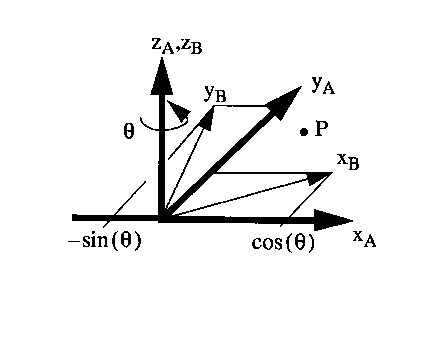
\includegraphics[width=3.5in]{figs02/00323.eps}
\caption{Two frames which are rotated relative to each other by the angle $\theta$ about the axis $z$.}\label{PlanarRotationFrames}
\end{figure}


Consider rotation in the $x,y$ plane about the axis $z$.  When we say ``about," we mean that any point along the line indicated by $z$ is unchanged by the rotation.  Also, the $z$ coordinate of any point is unchanged by rotation about the $z$ axis.  In Figure \ref{PlanarRotationFrames} we have two frames, $A$, in bold, and $B$.   $B$ is rotated about the $z$ axis with respect to $A$.   Consider the tip of the unit vector $x_A$.  After its rotation to $x_B$, it has components which we can project back on to $x_A$ and $y_A$.   It still has no component in $z$.   If we have rotated around $z$ by angle $\theta$, then these projections are
\[
^Ax_B = \left [ \begin{array}{c}   cos(\theta) \\ sin(\theta) \\ 0 \end{array} \right ]
\]
Similarly,

\[
^Ay_B = \left [ \begin{array}{c}   -sin(\theta) \\ cos(\theta) \\ 0 \end{array} \right ]
\]

These are two columns of the rotation matrix $^A_BR$:
\[
^A_BR = \left[
\begin{array}{ccc}
cos(\theta) & -sin(\theta) & ? \\
sin(\theta) &  cos(\theta) & ? \\
0           &          0   & ? \\
\end{array}\right]
\]


We can get column 3 of $^A_BR$ two ways.  First, as we have just done, we can note that
\[
^Az_B = {^Az_A} = \left[\begin{array}{c} 0 \\ 0 \\ 1 \end{array}\right]
\]
Therefore our complete matrix must be

\[
^A_BR = \left[
\begin{array}{ccc}
cos(\theta) & -sin(\theta) & 0 \\
sin(\theta) &  cos(\theta) & 0 \\
0           &          0   & 1 \\
\end{array}\right]
\]

A second way to complete the rotation matrix is to use definition 4, which specifies that the magnitude of each row or column must be one (Sec \ref{RotDefs}).  Thus
\[
|r_{31}|^2 = 1-\cos(\theta)^2-\sin(\theta)^2 = 0
\]
etc.

Our favorite point, $P$, has the representation $\{P_{XA}, P_{YA}\}$ in the $x,y$ plane.  $P_{ZA}$ can have any value for this discussion since our rotation is about $z$.
Just as it did with the unit vectors, $^A_BR$ maps $P$'s representation in $B$ to its representation in $A$:
\[
^AP = {^A_BR} \; {^BP}
\]
One way we can see this is by an argument of superposition since matrix multiplication is a linear transformation and $^BP$ can be expressed as a linear combination of the unit vectors of $B$.


%%%%** Sect
\subsection{Rotational Operators}
By similar arguments we can derive rotation matrices for rotation around the other axes, $x$, and $y$.  Let's denote the unit vectors,
\[
\hat{x} \equiv [1 \quad 0 \quad 0]^T \quad \hat{y} \equiv  [0 \quad 1 \quad 0 ]^T \quad \hat{z} \equiv [0 \quad 0 \quad 1]^T
\]
These are not vectors in any particular coordinate system, just the numerical values shown above.   We will define the matrices

\[
\mathrm{Rot}(\hat{x}, \theta) =  \left[
\begin{array}{ccc}
1  &     0        &      0    \\
0  &  \cos(\theta) & -\sin(\theta) \\
0  &  \sin(\theta) &  \cos(\theta) \\
\end{array} \right]
\]

\[
\mathrm{Rot}(\hat{y}, \theta) =  \left[
\begin{array}{ccc}
\cos(\theta)  &       0      & \sin(\theta) \\
     0       &       1      &     0       \\
-\sin(\theta) &       0      & \cos(\theta) \\
\end{array}\right]
\]

\[
\mathrm{Rot}(\hat{z}, \theta) =  \left[
\begin{array}{ccc}
\cos(\theta) & -\sin(\theta) & 0 \\
\sin(\theta) &  \cos(\theta) & 0 \\
0           &          0   & 1 \\
\end{array}\right]
\]



to designate rotations about the three main axes of a frame.   At this point let's introduce a shorter notation:

\[
c\theta \equiv cos(\theta), \quad s\theta \equiv sin(\theta)
\]
and
\[
c_1 = \cos(\theta_1), \quad s_1 = sin(\theta_1)
\]
for example,
\[
\mathrm{Rot}(\hat{x}, \theta_3) =
\left[
\begin{array}{ccc}
1  &  0  &  0    \\
0  & c_3 & -s_3  \\
0  & s_3 &  c_3  \\
\end{array}\right]
\]


\begin{ExampleSmall}
A point in frame $B$ is
\[
^BP = \left [ \begin{array}{c} -2 \\ 2 \\ 0.707 \end{array}\right]
\]
and there exists a frame $A$, whose rotation relative to $B$ is given by
\[
^A_BR = \mathrm{Rot} (\hat{x}, \pi/4 )
\]

1) What are the elements of $^A_BR$?

Answer:
\[
^A_BR = \left [ \begin{array}{ccc}
1  & 0 & 0  \\
0 & 0.707 & -0.707 \\
0 & 0.707 &  0.707 \end{array}\right]
\]

2) What is $^AP$?

Answer:
\[
^AP = ^A_BR{^BP} = \left[\begin{array}{c} -2.0 \\ 0.914 \\ 1.914 \end{array}\right]
\]

3) What is the change in magnitude of $P$ when it is rotated?

Answer:
\[
\frac{|^AP|}{|^BP|} = \frac{2.915}{2.915} = 1
\]


A rotation matrix should never change the magnitude of a point.
\end{ExampleSmall}



We can verify the fourth definition of the rotation matrix with the rotation operators. For example, using Rot($\hat{x}, \theta)$ we can easily verify that its columns have magnitude 1.   We can verify the cross product constraints as well. Using Rot($\hat{x}, \theta)$,  then let $a$ and $b$ equal the first two columns
\[
a = [1 \quad 0 \quad 0]^T, \quad b = [0 \quad c\theta \quad s\theta]^T
\]
We want to show that $a\times b=c$.
Recall that one definition of the vector cross product is
\[
a\times b = \left [
\begin{array}{ccc}
0 & -a_3 & a_2 \\
a_3 & 0 & -a_1 \\
-a_2 & a_1 & 0 \end{array} \right]
b
\]
so returning to our example,

\[
c = a \times b = \left [
\begin{array}{ccc}
0  & 0  & 0 \\
0  & 0 & -1 \\
0  & 1 & 0   \end{array} \right]
\left[ \begin{array}{c}
0 \\ c\theta \\ s\theta \end{array} \right]
=
\left[ \begin{array}{c}
0 \\ -s\theta \\ c\theta \end{array} \right]
\]

which is the answer we expect (i.e the third column of $\mathrm{Rot}(\hat{x},\theta)$) and  verifies that the third column is orthogonal to the first two.

%%%%** Section 4.2
\subsection{Inverse of a Rotation Matrix}

The properties given in our fourth definition describe an {\it orthonormal } matrix.   Any orthonormal matrix has an inverse which is equal to its transpose.  Thus for rotation matrices
\[
R^{-1} = R^T
\]
Clearly the inverse of a rotation matrix always exists because the transpose always exists.  When we apply this to  the coordinate transform application of rotation matrices:
\[
(^A_BR)^{-1} = (^A_BR)^T = ^B_AR
\]


%%%%** Section 4.3
\subsection{Composition of Rotations}\label{rotationorder}
Suppose there are two rotations which create a more complex relationship between two frames.  If we can transform a point from a rotated frame back to the base frame by premultiplying by the rotation matrix, then we should be able to do this twice to represent two rotations.




\begin{ExampleSmall}\label{RotExampLocalFrame}

Two frames, $A$, and $B$, start out coincident ($^A_BR = I$).  Then frame $B$ is rotated about $z_A$ by $\theta$ and then frame $B$ is rotated about $y_B$ by $\phi$.  Note that the second axis, $y_B$, is known in the most recent frame:
\[
^By_B = [0 \quad 1\quad 0]^T = \hat{y}
\]
.

1) What is $^A_BR(\theta,\phi)$?  In other words, what matrix represents the combination of both rotations?

Answer: Consider an intermediate frame, $A'$, to represent the frame after the first rotation:
\[
^A_{A'}R = \mathrm{Rot}(\hat{z}, \theta)
\]
by definition 3
\[
^{A'}_BR = \mathrm{Rot}(\hat{y},\phi)
\]
So now consider mapping a point in frame $B$, $^BP$, back to $A$ using definition 2 twice:
\[
^AP = {^A_{A'}}R {^{A'}_B}R ^BP
\]
Thus,
\[
^A_BR = \mathrm{Rot}(\hat{z},\theta)\mathrm{Rot}(\hat{y},\phi)
\]
\end{ExampleSmall}


We may combine successive rotations by {\it post}multiplication if each rotation is about a vector represented in the {\it current} rotated frame.
In  Example \thechapter.\ref{RotExampLocalFrame}, the first rotation, Rot$(\hat{z},\theta)$, is postmultiplied by the second rotation, $\mathrm{Rot}(\hat{y},\phi)$ to get the compound rotation $^A_BR$. This gives
\[
^A_BR(\theta, \phi) =
\left[
\begin{array}{ccc}
 c\theta & -s\theta & 0  \\
 s\theta &  c\theta & 0  \\
   0     &     0    & 1
\end{array}\right]
\left[
\begin{array}{ccc}
c\phi  & 0  & s\phi  \\
0      & 1  &   0    \\
-s\phi & 0  & c\phi
\end{array}\right]
=
\left[
\begin{array}{ccc}
c\theta c\phi       &     -s\theta      &  c\theta s\phi   \\
s\theta c\phi       &      c\theta      &  s\theta s\phi   \\
-s\phi              &         0         &   c\phi         \\
\end{array}\right]
\]




When successive rotations are described with respect to a single, fixed frame (in contrast to the compound example above), we may combine these by {\it pre}multiplication.   To illustrate this, we'll take the previous example of compound rotations and change just one thing:  the second rotation will take place around $y_A$ instead of $y_B$.




\begin{Example}\label{RotExampFixedFrame}

Two frames, $A$, and $B$, start out coincident ($^A_BR = I$).  Then frame $B$ is rotated about $z_A$ by $\theta$ and then frame $B$ is rotated about $y_A$ by $\phi$.  Unlike the previous example, the second axis is known only in the original frame, frame $A$. So we know:
\[
^By_A \ne [0 \quad 1 \quad 0]^T
\]


1) What is $^A_BR(\theta,\phi)$ this time?

\vspace{0.2in}

Answer: As before, consider the intermediate frame, $A'$, to represent the frame after the first rotation:
\[
{^A_{A'}}R = \mathrm{Rot}(\hat{z}, \theta)
\]
by definition 3 (Section \ref{RotDefs}).  For the second rotation let's use the point mapping interpretation, definition 2.  The second rotation must be represented by a matrix which maps a point from $B$ to $A'$.  This rotation is {\it not} one of our three cannonical rotation matrices because $y_A \ne \hat{y} $ in our current frame.   We can derive the proper transformation by breaking it down into three steps:


\begin{enumerate}
  \item Rotate (as  in physical move) $A'$ to $A$ using $^{^{A'}_{A}R}$.
  \item $\mathrm{Rot}(\hat{y},\phi)$
  \item Rotate back to $A'$ using $^{A}_{A'}R$.
\end{enumerate}
Thus,
\[
^{A'}_{B}R = \mathrm{Step\;1}\times\mathrm{Step\;2}\times\mathrm{Step\;3}
\]
\[
^{A'}_{B}R =  {{}^{A'}_A}R \; \mathrm{Rot}(\hat{y}, \phi) \; {}^A_{A'}R
\]

Now the complete mapping from $B$ to $A$ is
\[
{^A_B}R =  {^A_{A'}}R \; {^{A'}_B}R = {^A_{A'}}R \; {^{A'}_A}R \; \mathrm{Rot}(\hat{y}, \phi) \; {^A_{A'}}R
\]

Because ${^A_{A'}}R = {^{A'}_A}R^{-1}$, the first two rotation matrices cancel giving
\[
^{A}_BR = \mathrm{Rot}(\hat{y}, \phi)^A_{A'}R = \mathrm{Rot}(\hat{y}, \phi) \mathrm{Rot}(\hat{z}, \theta)
\]

expanding this:
\[
^A_BR = \begin{bmatrix} c\phi & 0 & s\phi \\ 0 & 1 & 0 \\ -s\phi & 0 & c\phi \end{bmatrix}
\begin{bmatrix}
c\theta      & -s\theta     &  0    \\
s\theta      &  c\theta     &  0    \\
   0         &     0        &  1
\end{bmatrix}
=
\begin{bmatrix}
c\phi c\theta     &  -c\phi s\theta    &  s\phi     \\
s\theta           &   c\theta          &  0         \\
-s\phi c\theta    &   s\phi c\theta    &  c\phi
\end{bmatrix}
\]

Note that after the cancelation, it is as though the second rotation {\it pre}multiplies the first one.

\end{Example}


\begin{Example}\label{RotExamp3Mixed}
Two frames $A$ and $B$ start out superimposed.  Then

\begin{quotation}

$B$ is rotated about $x_A$ by $\theta_1$.

$B$ is rotated about $y_B$ by $\theta_2$.

$B$ is rotated about $y_A$ by $\theta_3$.

\end{quotation}

What is $^A_BR$?

\vspace{0.2in}

Answer:

Set up intermediate frames as above:  $A', A''$.  Then
\[
^A_BR = {}^A_{A'}R \; ^{A'}_{A''}R \; ^{A''}_BR
\]

Considering the first rotation, since in the initial frame, $x_A = \hat{x}$ we can write
\[
^A_{A'}R = \mathrm{Rot}(\hat{x},\theta_1)
\]

In the second rotation, the axis is also known in the current frame: $^{A'}y_B=\hat{y}$, we can similarly write:
\[
^{A'}_{A''}R = \mathrm{Rot}(\hat{y},\theta_2)
\]

However for the third rotation we have to go all the way back to the initial frame:
\[
^{A''}_{B}R = \underbrace{
               ^{A''}_{A'}R \; ^{A'}_{A}R \; \mathrm{Rot}(\hat{y},\theta_3) \;  ^{A}_{A'}R \;^{A'}_{A''}R
               }
\]

Combining
\[
^A_BR = \underbrace{
     {}^A_{A'}R \; ^{A'}_{A''}R \;  ^{A''}_{A'}R \; ^{A'}_{A}R
     }_{=I}
\mathrm{Rot}(\hat{y},\theta_3) \;  ^{A}_{A'}R \;^{A'}_{A''}R
= \mathrm{Rot}(\hat{y},\theta_3) \;  ^{A}_{A'}R \;^{A'}_{A''}R
\]
\[
^A_BR = \mathrm{Rot}(\hat{y},\theta_3) \mathrm{Rot}(\hat{x},\theta_1) \mathrm{Rot}(\hat{y},\theta_2)
\]

\end{Example}


\begin{Example}

\begin{center}
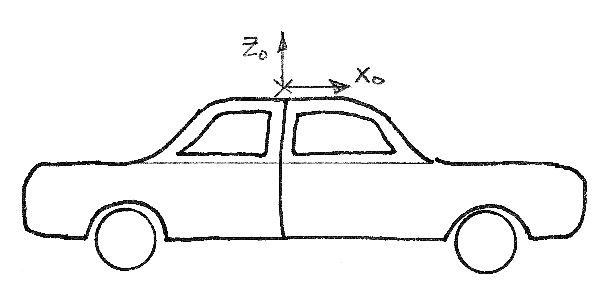
\includegraphics[width=3.5in]{figs02/00708.eps} ($\to$ front of car)
\end{center}
\vspace{0.2in}
A robotic car drives straight for 10 meters then turns right by $90^\circ$.  Then it drives up  a $45^\circ$ incline and comes to a stop.

A frame mounted to the top of the vehicle is called $F_0$.
The onboard computer can store the current value of $F_0$ at any time from navigation instruments as a 3x3 matrix.  Before driving the computer stores
\[
F_1 = F_0
\]
Then after the drive above, it stores the new orientation,
\[
F_2 = F_0
\]


What is the rotation matrix ${^1_2R}$ which describes the change in orientation?

Answer:

We have rotation matrices describing the three stages of the trip:

1) Drive straight for 10 meters:  $\begin{bmatrix}  1 & 0 & 0 \\ 0 & 1 & 0 \\ 0 & 0 & 1 \end{bmatrix}$

2) Turn right by $90^\circ$: Rot($\hat{z}$,  $-90^\circ$):  $\begin{bmatrix} 0 & 1 & 0 \\ -1 & 0 & 0 \\ 0 & 0 & 1 \end{bmatrix}$

3) Go up $45^\circ$ incline: Rot($\hat{y}, -45^\circ)$:  $\begin{bmatrix} 0.707 & 0  & -0.707 \\ 0 & 1 & 0 \\ 0.707 & 0 & 0.707 \end{bmatrix}$\\
(about the {\it local } frame).

Then we can combine them by postmultiplication:
\[
{^1_2R} = \begin{bmatrix}  1 & 0 & 0 \\ 0 & 1 & 0 \\ 0 & 0 & 1 \end{bmatrix}
\begin{bmatrix} 0 & 1 & 0 \\ -1 & 0 & 0 \\ 0 & 0 & 1 \end{bmatrix}
\begin{bmatrix} 0.707 & 0  & -0.707 \\ 0 & 1 & 0 \\ 0.707 & 0 & 0.707 \end{bmatrix}
\]
\[
{^1_2R} = \begin{bmatrix} 0 &  1 & 0 \\ -0.707 & 0 & 0.707 \\ 0.707 & 0 & 0.707 \end{bmatrix}
\]


\end{Example}

It can be confusing to remember the order of multiplication for multiple rotations.   One way to think about it is we always post-multiply successive rotations.  If the rotation is about the first, fixed frame, then we must use the similarity transformation as shown in Examples \ref{RotExampFixedFrame} and \ref{RotExamp3Mixed} of this chapter.  The effect of this similarity transformation is to make this appear like pre-multiplication.


To summarize, if we are careful, we can use the following rules of thumb to determine the order of matrix multiplication:

\begin{enumerate}
  \item  If the rotation is about an axis in the {\it original fixed  } frame, pre-multiply
  \item  If the rotation is about an axis in the {\it current} frame, post-multiply
\end{enumerate}



%%%%** Section 4.4
\subsection{Rotation of a Point}
The rotation matrix also describes the physical act of turning something (Figure \ref{RotationOfAPoint}).   So how can we describe the rotation of a point about an axis in a certain frame but still representing the point in the same frame?


%%%%** Figure 3
\begin{figure}
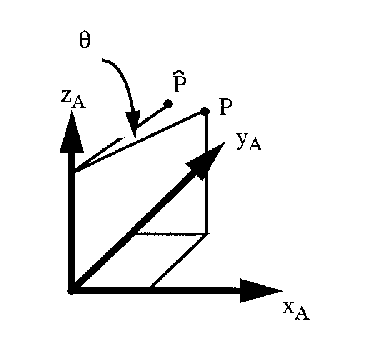
\includegraphics[width=3.0in]{figs02/00324.eps}
\caption{Rotation of a point around the $z$ axis by angle $\theta$.   Here we consider the point to actually move in a single frame, $A$. }\label{RotationOfAPoint}
\end{figure}

We consider the point's rotation to be positive if the angle from the orginal point, $P$, to the rotated point, $\hat{P}$, is positive in the right hand sense around the axis.  Consider for example, rotation of the point around the $\hat{z}$ axis.    By our third definition (Section \ref{RotDefs}),
\[
^A\hat{P} = \mathrm{Rot}(\hat{z},\theta)^AP
\]




%%%%** Section 4.5
\subsection{Rotations about axes other than $x,y,z$}
Suppose we have an arbitrarily rotated frame, F:
\[
F = {}^O_FR
\]
Geometrically, this might look like Figure \ref{ArbitraryRotation}.   Now we will use frame $F$ to study more general rotations.   Suppose $ ^O_FR$ is known and we want to do a rotation about $z_F$?  How do we represent a rotation about $z_F$ in frame $O$ by $\theta$?   Put another way, if the point $^OP$ is rotated about $z_F$ by $\theta$ to get $^O\hat{P}$, what is $^O\hat{P}$?

We solve this similarly to the last example by transforming back to frame $F$ and doing the canonical rotation about $\hat{z}$:
\[
^O\hat{P} = \;{}^O_FR \mathrm{Rot} \left (
\begin{bmatrix}  0 \\ 0 \\ 1 \end{bmatrix} , \theta \right )
 {}^F_OR
\]

\[
= \mathcal{R} \mathrm{Rot}(\hat{z},\theta)\mathcal{R}^T \; ^OP
\]
where $\mathcal{R} \equiv \;{}^O_FR$.
Another way to look at this is to define

\[
\mathrm{Rot}(z_F,\theta) = \mathcal{R} \mathrm{Rot}(\hat{z},\theta)\mathcal{R}^T
\]

Mathematically, this is a ``similarity transform" which can be used to rotate about an arbitrarily rotated vector, in this case, $z_F$.




%%%%** Figure 4
\begin{figure}
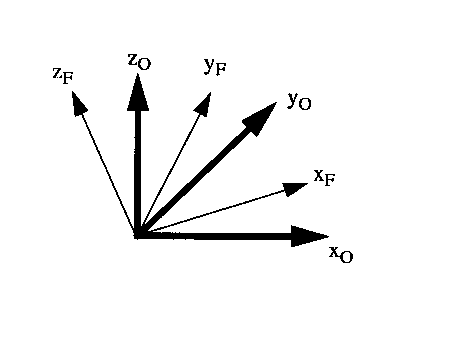
\includegraphics[width=3.5in]{figs02/00326.eps}
\caption{Frame $F$ has an arbitrary orientation relative to frame $O$}\label{ArbitraryRotation}
\end{figure}






%%%%** Section 5
\section{Three Parameter Representations of Rotation}
Although nine numbers are required to make a rotation matrix, only 3 of them are independent (this is because there are six constraints on the matrix in definition 4 of Section \ref{RotDefs}).  This implies that there should be representations of rotation needing only 3 parameters.


%%%%** Section 5.1
\subsection{Roll-Pitch-Yaw Angles (XYZ Fixed Angles)}

%%%%** Figure 5
\begin{figure}
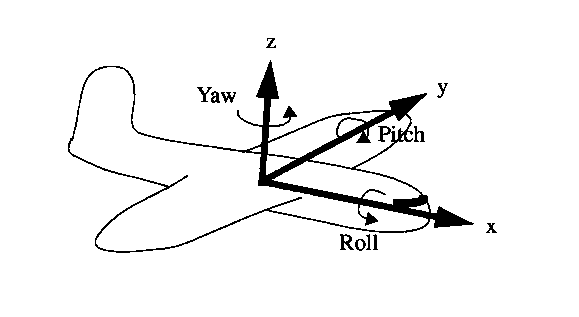
\includegraphics[width=3.5in]{figs02/00327.eps}
\caption{Roll-Pitch-Yaw angles (commonly used in avaition) describe rotations in a fixed order about $x,y,z$ axes of a fixed coordinate system.}\label{RollPitchYawFig}
\end{figure}

In aviation, aeronautics and sailing, the terms ``roll, pitch, and yaw" are commonly used.  These terms describe rotations about the $x,y,z$ axes of a fixed coordinate system in that order (Figure \ref{RollPitchYawFig}).  When we say that the coordinate system is ``fixed," we mean {\it not } that it is fixed to the object (i.e. the aircraft of Figure \ref{RollPitchYawFig}), but that its orientation is fixed in space.  Following the argument of Section \ref{rotationorder}, since these rotations are about a fixed frame, they should be combined by {\it pre-multiplication}:
\begin{equation}\label{RPYeqn}
R_{RPY} = \mathrm{Rot}(\hat{z}, Yaw)  \mathrm{Rot}(\hat{y}, Pitch)  \mathrm{Rot}(\hat{x}, Roll)
\end{equation}
If we define the amounts of Roll, Pitch, and Yaw, (positive in the right hand sense) about $x,y,z$ to be $C, B, A$ respectively, then
\[
R_{RPY} = \mathrm{Rot}(\hat{z}, A)  \mathrm{Rot}(\hat{y}, B)  \mathrm{Rot}(\hat{x}, C)
\]
\[
=
\begin{bmatrix}
 cA   & -sA  &  0    \\
 sA   &  cA  &  0    \\
 0    &   0  &  1
\end{bmatrix}
\begin{bmatrix}
cB    &  0   &  sB  \\
0     &  1   &  0   \\
-sB   &  0   &  cB
\end{bmatrix}
\begin{bmatrix}
 1    &  0   &   0  \\
 0    &  cC  &  -sC \\
 0    &  sC  &  cC
\end{bmatrix}
= \begin{bmatrix}
cAcB  &  cAsBsC-sAcC    &  cAsBcC+sAsC   \\
sAcB  &  sAsBsC+cAcC    &  sAsBcC-cAsC   \\
-sB   &  cBsC           &    cBcC
\end{bmatrix}
\]



%%%%** Section 5.2
\subsection{ZYX Euler Angles}\label{ZYXEuler}


Another 3-parameter representation which is commonly used is Euler Angles.
In this case the rotations are taken about the axes of a {\it rotating} frame.
Start with $F_1 = \{x_1,y_1,z_1\}$ superimposed on $F_0$.  Then rotate through the three steps labeled A-C in Figure \ref{ZYXEulerRotations}.

\begin{enumerate}
  \item Rotate about $z_0$ by $A$ to create $F_1$.
  \item Rotate about $y_1$ by $B$ to create $F_2$.
  \item Rotate about $x_2$ by $C$ to create $F_3$.
\end{enumerate}

By definition (3), step one defines $^0_1R$, step two defines $^1_2R$, etc.  By definition (2)
\[
^0_1R = \mathrm{Rot}(\hat{z},A) =
\mathrm{Rot} \left (
\hat{z} , A \right )
\]
maps a point in frame 1 to frame 0.
\[
^1_2R = \mathrm{Rot}(\hat{y},B) =
\mathrm{Rot} \left (
\hat{y} , B \right )
\]
maps a point in frame 2 to frame 1. And
\[
^2_3R = \mathrm{Rot}(\hat{x},C) =
\mathrm{Rot} \left (
\hat{x} , C \right )
\]
maps a point in frame 3 to frame 2.

Using the point mapping interpretation, the complete mapping is
\begin{equation}\label{ZYXEulerEqn}
^0_3R = ^0_1R\;^1_2R\;^2_3R = \mathrm{Rot}(\hat{z},A)\mathrm{Rot}(\hat{y},B)\mathrm{Rot}(\hat{x},C)
\end{equation}
Note that \eqref{RPYeqn} is the same as \eqref{ZYXEulerEqn}.   But, the Roll Pitch and Yaw angles are {\it not} equivalent to ZYX Euler angles, because the rotations $A$, $B$, and $C$ were applied in opposite orders in the two cases.  Specifically, for roll-pitch-yaw angles, we used $C$ for roll, but roll is applied {\it first} in the RPY method.
%%%%** Figure 6
\begin{figure}[h]
A 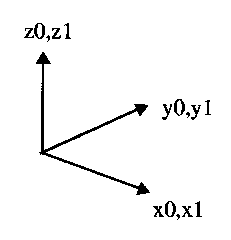
\includegraphics[width=1.0in]{figs02/00328.eps}
B 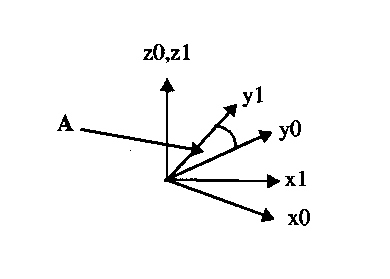
\includegraphics[width=1.5in]{figs02/00329.eps}
C 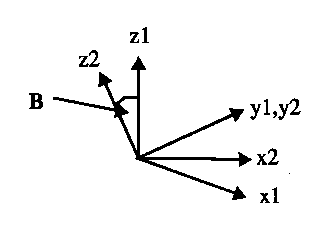
\includegraphics[width=1.5in]{figs02/00330.eps}
D 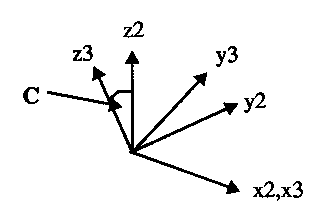
\includegraphics[width=1.5in]{figs02/00331.eps}
\caption{Initial Frames and rotations which make up the ZYX Euler Angles.}\label{ZYXEulerRotations}
\end{figure}
%
%
% %%%%** Section 5.3
% \subsection{ZYZ Euler Angles}
%
%
% (Similar material to previous subsection on ZYX Euler Angles)


%%%%** Section 6
\section{Equivalent Angle-Axis}\label{EquivAngleAxis}

Euler proved that any state of 3D rotation can be expressed by a single axis (i.e. a unit vector) and an amount of rotation.
Let the axis of rotation be
\[
K = [K_X\quad K_Y\quad K_Z]^T
\]
and the amount of rotation (in the right hand sense around $K$) be $\theta$,
then
\[
R_{K\theta} =
\begin{bmatrix}
K_X^2v\theta+ c\theta		& K_XK_Yv\theta-K_Zs\theta		&K_XK_Zv\theta+K_Ys\theta \\
K_XK_Yv\theta+K_Zs\theta	& K_Y^2v\theta+c\theta			&K_YK_Zv\theta-K_Xs\theta \\
K_XK_Zv\theta-K_Ys\theta	& K_YK_Zv\theta+K_Xs\theta		&K_Z^2v\theta+c\theta
\end{bmatrix}
\]
where
\[
v\theta = 1-\cos(\theta) \qquad c\theta = \cos(\theta) \qquad s\theta=\sin(\theta)
\]
Also, we require that $|K|=1$ to obtain a valid rotation matrix.   If implementing 
$R_{K\theta}$ in software, it is a good idea to normalize $K$ first as in:

\[
K = \frac{K}{|K|}
\]
so that we are sure it has magnitude 1. 

\begin{ExampleSmall}
Work out $R_{K\theta}$ for the special case of the $Z$ axis and compare the result to $rot(\hat{z}, \theta)$.

Let
\[
K = [0\quad0\quad1]^T
\]
Then setting $K_X$ and $K_Y$ to zero,
\[
R_{K\theta} =
\begin{bmatrix}
c\theta				& -K_Zs\theta				& 0 \\
K_Zs\theta			&     c\theta				& 0 \\
0				& 0					&K_Z^2(1-c\theta)+c\theta
\end{bmatrix}
\]
Since $K_Z=1$, this is equivalent to $rot(\hat{z}, \theta)$.
\end{ExampleSmall}


%%%%** Section 7
\section{Quaternions}\label{QuaternionSection}

% When we study Inverse Kinematics (Chapter \ref{xxxxxxxx}), we will see that there are difficulties with these three-parameter representations of rotation at certain configurations (for example when $B=0$).   An alternative is available which uses four parameters to represent orientation which has a  well defined representation for every orientation.   This alternative uses the notion of quaternions.

Another way to represent rotations of rigid bodies uses quaternions, a system like complex numbers which uses three ``imaginary" variables instead of just $i$.

To understand how a quaternion represents rotations, first consider basic complex numbers of the form $M = a+bi$.   The real and imaginary components of $M$ form a point in the complex plane.  For the purposes of rotation, we can assume that the magnitude of $M$ is 1 ($|M|=1$).  In polar form,
\[
|M| = \sqrt{a^2+b^2}  \qquad \angle{M} = \mathrm{atan2}(a,b)
\]

Remembering the rule ``Angles add, magnitudes multiply," or
\[
\angle(MN) = \angle(M) + \angle(N)
\]

Since $|M|= 1$, we can think of multiplying a complex number by $M$ as an operator which rotates the point to a new angle.
Electrical engineers will be familiar with this concept used to describe phase relationships between AC signals of the same frequency (phasors).

Quaternions can be thought of as a generalization of complex numbers using the symbols $i, j,$ and $k$, where
\[
i^2 = j^2 = k^2 = ijk = -1
\]
and where the multiplication of these elements is NOT commutitive (i.e. $ij \neq ji$).  The ``quaternion" has three imaginary components and one real component:
\[
q = a + bi+cj+dk
\]
The quaternion $q$ can also be thought of as the sum of a scalar ($a$) and a vector ($bi+cj+dk$).

Just as a complex number $M=a+bi$ has a complex conjugate, $M^* = a - bi$, quaternions have a quaternion conjugate

\begin{equation}\label{quaternioninversedefinition}
q^* = a - (bi+cj+dk)
\end{equation}

Just as a normal complex number can represent a rotation in the plane, quaternions can represent rotations in three dimensions.  The rotation is described by an axis of rotation, $K$, and a degree of rotation $\theta$.   As we saw above in Section \ref{EquivAngleAxis}, any rotation can be expressed this way as long as $\theta \neq 0$.

The well-known Euler's forumula for complex numbers is
\[
e^{i\theta} = \cos(\theta) + i\sin(\theta)
\]
The corresponding formula for quaternions is
\[
e^{\alpha(a_xi+a_yj+a_zk)} = \cos(\alpha) + (a_xi+a_yj+a_zk)\sin(\alpha)
\]
To use this to represent rotations we set $\alpha = \theta/2$.  Thus for an axis of rotation $K = (K_x, K_y, K_z)$
the quaternion representation of a rotation by $\theta$ around the axis $K$ is
\[
q = e^{\frac{\theta}{2} (K_xi+K_yj+K_zk)} = \cos(\theta/2) + (K_xi+K_yj+K_zk)\sin(\theta/2)
\]

The magnitude of $K$ is not used for rotation and often we require $|K|=1$.  The resulting quaternion is a unit quaternion.

To represent this quaternion without using $i,j,k$ (for example in some software), we just write down the four components

\begin{equation}\label{quaterniondefinition}
q = \cos(\theta/2) + K_xi\sin(\theta/2)+K_yj\sin(\theta/2)+K_zk\sin(\theta/2) = [w,x,y,z]
\end{equation}

\[
w = \cos(\theta/2) \qquad x =  K_x\sin(\theta/2) \qquad y = K_y\sin(\theta/2) \qquad z = K_z\sin(\theta/2)
\]
\begin{equation}\label{quaternioncomponents}
q = [w,x,y,z]
\end{equation}

Multiplication of quaternions is best left to the computer!  If two quaternions are given by
\[
q_1 = a_1 + b_1i + c_1j + d_1k \qquad q_2 = a_2 + b_2i + c_2j + d_2k
\]
Their product is
\begin{equation}\label{quaternionproduct}
q_{12} =
 a_1a_2-b_1b_2-c_1c_2-d_1d_2 +
(a_1b_2+b_1a_2+c_1d_2-d_1c_2)i +
(a_1c_2-b_1d_2+c_1a_2+d_1b_2)j +
(a_1d_2+b_1c_2-c_1b_2+d_1a_2)k
\end{equation}
or equivalently
\[
q_{12} =   \begin{array}{ccc}
[ a_1a_2-b_1b_2-c_1c_2-d_1d_2, &
(a_1b_2+b_1a_2+c_1d_2-d_1c_2),&
(a_1c_2-b_1d_2+c_1a_2+d_1b_2),\\
\qquad (a_1d_2+b_1c_2-c_1b_2+d_1a_2) ]
\end{array}
\]
whenever we write the product of two quaternions (i.e. $q_1q_2$) we refer to this computation (which, like matrix multiplication, is not commutative).


The quaternion can be expressed as a rotation matrix as follows

\[
R(q) =  \begin{bmatrix}
 c\theta	+ K_x^2(1-c\theta)	&  K_xK_y(1-c\theta) -K_zs\theta 	&  K_xK_z(1-c\theta)+K_ys\theta \\
K_yK_x(1-c\theta)+K_zs\theta	&  c\theta+K^2_y(1-c\theta)       &  K_yK_z(1-c\theta)-K_xs\theta   \\
K_zK_x(1-c\theta)-K_ys\theta	&  K_zK_y(1-c\theta)+K_xs\theta	&  c\theta+K_z^2(1-c\theta)      \\
\end{bmatrix}
\]
where $s\theta = \sin(\theta)$ and $c\theta = \cos(\theta)$.
Equivalently, for $q = [w,x,y,z]$,

\[
R(q) = \begin{bmatrix}
1-2y^2-2z^2	& 2(xy-wz)	& 2(wy+xz)	\\
2(wz+yx)	& 1-2x^2-2z^2	& 2(yz-xw)	\\
2(xz-wy)	& 2(yz+xw)	& 1-2y^2-2x^2
\end{bmatrix}
\]

Since each quaternion corresponds to a rotation matrix, combining successive rotations represented by quaternions should be done in the same order as combining rotation matrices.   I.e. if the next rotation is expressed as a quaternion in the local coordinate system, post-multply and if it is expressed in a fixed original coordinate system, pre-multiply.

\begin{ExampleSmall}\label{quaternionmultiplication}
Two frames $A$ and $B$, are initially aligned.  Frame $B$ is first rotated by $30^\circ$ about the vector $[0.371, 0.557, 0.743]$.
Then Frame $B$ is further rotated by $45^\circ$ about the vector $[0.684, 0.570, 0.456]$ (in the current frame).  Find the quaternion representing the complete rotation.

\[
q_1 = [ \cos(15^\circ), \quad 0.371\sin(15^\circ), \quad 0.557\sin(15^\circ), \quad 0.743\sin(15^\circ)]
\]
\[
q_2 = [ \cos(22.5^\circ), \quad 0.684\sin(22.5^\circ), \quad 0.570\sin(22.5^\circ), \quad 0.456\sin(22.5^\circ)]
\]
\[
q_{12} = q_1q_2
\]
Using the computer:
\[
q_1 = [0.966, 0.096, 0.144, 0.193] \qquad  q_2 = [0.924, 0.262, 0.218, 0.174]
\]
\vspace{0.1in}
\[
q_{12}= q_1q_2 = [0.802 \quad 0.325, \quad 0.377 \quad 0.330]
\]

\end{ExampleSmall}

\begin{ExampleSmall}


A rotation is to be performed about the vector $Rv = (0,1,0)$ by $45^\circ$.    Compute the quaternion to represent this rotation, and express it as a Rotation matrix.

\vspace{0.1in}

First, $\theta$ = $45^\circ$, and the axis of rotation, $K = [0,1,0]$, so using equation \ref{quaternioncomponents},

\[
q = [\cos(\theta/2), \quad 0\sin(\theta/2),\quad 1\sin(\theta/2),\quad 0\sin(\theta/2) ]
\]
\[
q = [.924, \quad 0, \quad .383, \quad 0]
\]
Using either matrix form above,
\[
R(q) = \begin{bmatrix}
0.707   &  0  &  0.707   \\
0       &  1  &  0       \\
-0.707   &  0  &  0.707   \\
\end{bmatrix}
\]

Which is the expected result since $q$ represents a rotation of $45^\circ$ about the $y$ axis.
\end{ExampleSmall}


\begin{Example}
Using the quaternions $q_1$ and $q_2$ from Example \thechapter.\ref{quaternionmultiplication}, Compute their two rotation matrices, multiply them together, and compare the result with the matrix version of $q_{12}$ from Example \thechapter.\ref{quaternionmultiplication}.

\vspace{0.1in}

First, convert $q_1$, $q_2$ to rotation matrices:
\begin{verbatim}

-->Ra = quat2rot1(qtimes(q1,q2))
 Ra  =

    0.4988392  - 0.2837947    0.8199695
    0.7742173    0.5728992  - 0.2723774
  - 0.3917614    0.7701054    0.5051711

-->Rb = quat2rot1(q1) * quat2rot1(q2)
 Rb  =

    0.4987583  - 0.2839447    0.8202152
    0.7744610    0.5728083  - 0.2725517
  - 0.3919257    0.7703584    0.5050751

\end{verbatim}

Comparing the results we see that the two matrices are nearly identical. More precisely, we can subtract the two matrices and find the maximum absolute error:
\begin{verbatim}

-->max(abs(Rb-Ra))
 ans  =

    0.0002530

\end{verbatim}
Since the columns and rows of rotation matrices must have magnitude 1, we can see that this error is very small.
\end{Example}


The inverse of a rotatation is the conjugate of the corresponding quaternion.  If $q$ is defined as in equation (\ref{quaterniondefinition}), then

\[
q^* = \cos(\theta/2) - K_xi\sin(\theta/2) -K_yj\sin(\theta/2) - K_zk\sin(\theta/2) = [w,-x,-y,-z]
\]


To use a quaternion for rotation of a point, if we define a point $P_1 = (P_x,P_y,P_z)$.  To rotate it around axis $K$ by $\theta$, let
\[
q_1 =  \cos(\theta/2) + (K_xi+K_yj+K_zk)\sin(\theta/2)
\]
and then
\begin{equation}\label{quaternpointrotation}
P_2 = q_1\hat{P}q_1^*
\end{equation}
where
\[
\hat{P} = [0,\; P_X,\; P_Y,\; P_Z]
\]
and the products are formed by quaternion-style multiplication.


\begin{ExampleSmall}
A rotation defined by a $63^\circ$ rotation about the axis $[-0.349, 0.814, 0.465]$ is applied to the point,
$P2 = [52.3, 67.0, -48.72]$.   Find the new point using quaternions and compare it with the equivalent angle-axis method.

\vspace{0.2in}

Using equation \thechapter.\ref{quaternpointrotation},
\begin{verbatim}
-->q4=quaternion([-.349,.814, .465], 63)
 q4  =

    0.8526402
  - 0.1822953
    0.4251816
    0.2428863

-->P2=[52.3,67,-48.72]
 P2  =

    52.3    67.  - 48.72

--> P2a = qtimes(q4, qtimes([0,P2],qcomp(q4)))
 P2a  =
    0.
  - 41.927377
    42.98847
  - 77.408106

// check by matrix rotation of point P2

-->R=quat2rot1(q4)
 R  =

    0.5204537  - 0.5692065    0.6364998
    0.2591720    0.8155493    0.5174062
  - 0.8136079  - 0.1043230    0.5719780

-->R*P2'
 ans  =
  - 41.927377
    42.98847
  - 77.408106

\end{verbatim}
\end{ExampleSmall}









%%%%** Section 8
\section{Side Topic:  Rotations in higher dimensions}
We have seen that at least three parameters are sufficient and necessary to specify rotation in three dimensions.   Is it a coincidence that 3 dimensional space has 3 rotation parameters?    Any hope for this simple rule is dashed by considering that only 1 orientation parameter is needed in 2 dimensions.   How many parameters are required to specify rotations of a 4 dimensional object?

We will use definition 4 to rephrase and generalize the question:  How many parameters does it take to specify an $n\times n$ orthonormal matrix?

The total number of matrix elements is $n^2$.   Then there are two sets of constraints:

\begin{enumerate}
  \item  $C_i \cdot C_j = 0$
  \item $|C_i| = 1$
\end{enumerate}
where $C_i$ is the $i$th column of the matrix.

The number of constraints due to the first condition is
\[
\binom{n}{2} = \frac{n!}{2(n-2)!}
\]
and the number of constraints of the second type is $n$.  So the total number of parameters is the number of matrix elements minus the number of constraints:
\[
N = n^2 - \frac{n!}{2(n-2)!}
\]
which can be simplified to
\[
N = \frac{1}{2} (n^2-n)
\]
So for a four dimensional object we need 6 parameters and for a 10 dimensional one we need 45 parameters(!).








%%%%** Section 9
\section{Homogeneous Transformation}
Considering several nice properties of the Rotation Matrix, in this Section, we will
find a  way to add translation to our matrix description of the configuration of a rigid object.
Earlier we used the $x,y,z$ coordinates of the origin of a frame attached to an object, with the rotation matrix of that frame,  to have its configuration completely specified  relative to some ``base frame," $B$ i.e.
\[
\mathrm{configuration} = \{^Bx,^By,^Bz, {}^B_0R\}
\]

More generally, this gives us a way to relate frames to each other.   Suppose we have a series of frames with different positions and orientations, and some relations between them as in Figure \ref{ThreeFramesVectors}.





%%%%** Figure 7
\begin{figure}
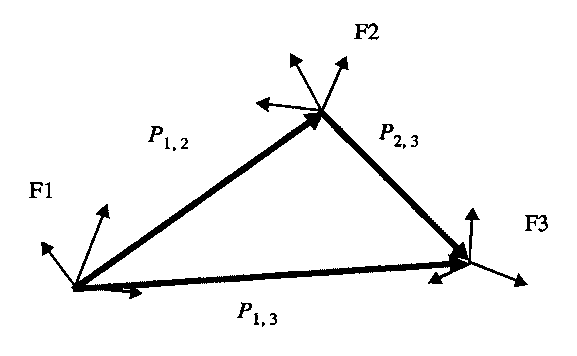
\includegraphics[width=3.5in]{figs02/00332.eps}
\caption{Three frames which are offset from each other in position and orientation. Vectors show displacements between the origins of the frames.}\label{ThreeFramesVectors}
\end{figure}



We can pose the following questions about these three frames:

If we know $P_{1,2}, P_{2,3}, \;^1_2R, \; ^2_3R$, what is $P_{1,3}, \;^1_3R$?

Consider a point expressed in frame 3, $^3P$.  It can be expressed in frame 2 by the affine transformation
\[
^2P = P_{2,3}+ \;{}^2_3R \;{}^3P
\]
and in frame 1 by
\[
^1P = P_{1,2} + \;{}^1_2R(P_{2,3}+ \;{}^2_3R \;{}^3P)
\]
Equivalently,
\[
^1P = \underbrace{P_{1,2} + ^1_2RP_{2,3}}{}+ \underbrace{^1_2R\;^2_3R}{} ^3P
\]
from which we can conclude
\[
P_{1,3} = P_{1,2} + ^1_2RP_{2,3} \qquad  ^1_3R = \;{}^1_2R\;^2_3R
\]


Although the preceding can be used as a general way to represent the spatial relationships between objects and robots, it is messy because we must add as well as multiply.  This is a problem because we often have to represent a series of these transforms which yields ever more complicated expressions.

An alternative is presented by ``homogeneous coordinates" which cleverly use an additional dimension to reduce the affine transformation to pure matrix multiplication.  We define the homogeneous transform
\[
^1P = \;{}^1_2T^2P
\]
where
\[
^1_2T =
\begin{bmatrix}
\begin{bmatrix}  &  &  \\  & ^1_2R&  \\ & & \\ \end{bmatrix}      &
 \begin{bmatrix}  \\ ^1P_{1,2} \\  \\ \end{bmatrix}            \\
 0 \quad 0 \quad 0      &   1
\end{bmatrix}
\]

This $4\times4$ matrix compactly describes both the rotation and the position offset.  When we work with homogeneous transforms, we augment our position vectors by adding a 1 in the fourth position. i.e.
\[
^1P = \begin{bmatrix} ^1P_x \\^1P_y \\ ^1P_z \\ 1 \end{bmatrix}
\]
in the example above,
\[^1P = ^1_2T^2P =
\begin{bmatrix}
\begin{bmatrix}  &  &  \\  & ^1_2R&  \\ & & \\ \end{bmatrix}      &
 \begin{bmatrix}  \\ ^1P_{1,2} \\  \\ \end{bmatrix}            \\
 0 \quad 0 \quad 0      &   1
\end{bmatrix}
\begin{bmatrix} ^2P_x \\^2P_y \\ ^2P_z \\ 1 \end{bmatrix}
\]
\[
= \begin{bmatrix}
^1_2R_{[1]}\cdot{}^2P+\;{}^1P_{{1,2}_{[1]}} \\
^1_2R_{[2]}\cdot{}^2P+\;{}^1P_{{1,2}_{[2]}} \\
^1_2R_{[3]}\cdot{}^2P+\;{}^1P_{{1,2}_{[3]}} \\
1\\
\end{bmatrix}
=
\begin{bmatrix}
^1P_{1,2}+ \;{}^1_2R \;{}^2P \\ 1 \\
\end{bmatrix}
\]

where $^1_2R_{[i]}$ represents row $i$ of $^1_2R$, and $^2P+\;{}^1P_{{1,2}_{[i]}}$ represents the $i$th element of $^1P_{1,2}$.
Notice that the final expression is completely equivalent to multiplying by a rotation matrix and then adding a translation.

With homogeneous transformations at our disposal, a series of spatial replationships can be expressed by a series of matrix multiplications as with pure rotation.  For example, solving the problem posed above for the three frames, $F1, F2, F3$,
\[
^1_3T = \; {}^1_2T\;^2_3T
\]
which is more compact indeed.

\paragraph{Homogeneous Transformation Definitions}\label{HTDefs}
The homogeneous transformation has definitions analogous to those we made for rotation:


The homogeneous transformation $^A_BT$ is

\begin{enumerate}
  \item A matrix which specifies frame $B$ in terms of frame $A$.
  \item A matrix which maps a point represented in frame $B$, $^BP$, to its representation in frame $A$, $^AP$.
  \item A description of an operator, perhaps corresponding to a physical move, {\it from} frame $A$, {\it to} frame $B$.
  \item A $4\times 4$ matrix with the structure given above.
\end{enumerate}


\begin{Example}
\begin{center}
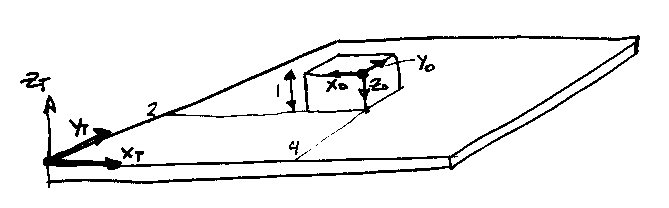
\includegraphics[width=4.5in]{figs02/00333.eps}
\end{center}

Find the $4\times 4$ homogeneous transformation which represents the configuration of the box on the table.   Frame $0$ is placed on a corner of the box and frame $T$ is at a corner of the table such that $X_T$ and $Y_T$ are in the plane of the table top.

Question:  What is $^T_0T$?

Answer:  First, find the translation offset between the origin of the box frame ($O$) and the table frame ($T$):
\[
^TP_O = \begin{bmatrix} 4 \\ 2 \\ 1 \end{bmatrix}
\]
Then, identify the rotation matrix.  First, align the frames by redrawing frame $O$ without the offset superimposed on $T$.  Then write each column of $^T_OR$.  Each column is the vector $\{x_O, y_O, z_O\}$ written in frame $T$:
\[
^T_OR = \begin{bmatrix}
-1 & 0 & 0 \\
0 & 1 & 0  \\
0 & 0 & -1 \\
\end{bmatrix}
\]
The homogeneous transform is thus:
\[\begin{bmatrix}
 -1   &   0  &  0  &  4  \\
  0   &   1  &  0  &  2  \\
  0   &   0  &  -1 &  1  \\
  0   &   0  &   0 &  1  \\
\end{bmatrix}
\]
\end{Example}

\begin{Example}

\includegraphics[width=4.5in]{figs02/00578.eps}

Two frames are on a conveyor belt.  We have the following facts about the system
\begin{itemize}
  \item The belt runs at 0.5 meters/sec.
  \item The belt is in the $\{X_0,Y_0\}$ plane.
  \item The belt is oriented $45^\circ$ from the $X_0$ axis as shown in the ``Top View".
  \item The origin of Frame $F_1$ is aligned with the origin of $F_0$ at $t=0$.
  \item Frame $F_1$ moves with the belt but Frame $F_0$ does not.
  \item $X_1$ is pointing along the belt (same direction as belt velocity.)
\end{itemize}

Find the 4x4 homogenous transform (which is a function of time) of $F_1$

Answer:

$O$:  The origin of $F_1$ is a function of time moving along the belt.
\[
O = \begin{bmatrix} 0.5t \cos(45^\circ) \\ 0.5t\sin(45^\circ) \\ 0 \end{bmatrix} = [0.35t, \quad 0.35t, \quad 0]^T
\]
Rotation = $rot(\hat{z}, 45^\circ)$
\[
\begin{bmatrix} 0.707 & -0.707 & 0 \\ 0.707 & 0.707 & 0 \\ 0 & 0 & 1 \end{bmatrix}
\]
\[
{^0_1T} = \begin{bmatrix} 0.707 & -0.707 & 0 & 0.35t \\ 0.707 & 0.707 & 0 & 0.35t \\ 0 & 0 & 1 & 0 \\ 0 & 0 & 0 & 1 \end{bmatrix}
\]
\end{Example}


%%%%** Section 9.1
\subsection{Inverse of Homogeneous Transforms}

We will frequently need the inverse of the 4x4 homogeneous transform matrix.   It seems intuitive that this inverse always exists because physical rotations and translations can always be ``undone."   It is straightfoward to derive the inverse of the 4x4 homogeneous transform,

Consider mapping a point in frame $B$ to its value in frame $A$ with both translation and rotation:
\[
^AP = {^A_BT}{^BP} = {^AO} + {^A_BR}{^BP}
\]
Where ${^AO}$ is the origin of frame $B$ expressed in $A$.
To invert this we seek a 4x4 matrix, $({^A_BT})^{-1}$ such that
\[
{^BP} = ({^A_BT})^{-1} {^AP}
\]

Solving
\[
{^BP} = ({^A_BR})^{-1}({^AP}-{^AO})
\]
\[
= {^B_AR} \; {^AP}-{^B_AR}\;{^AO}
\]
% Thus,
% \[
% T  =
% \begin{bmatrix}
% \begin{bmatrix}  &  &  \\  & R &  \\ & & \\ \end{bmatrix}      &
%  \begin{bmatrix}  \\  P \\  \\ \end{bmatrix}            \\
%  0 \quad 0 \quad 0      &   1
% \end{bmatrix}
% \]
% is
\[
{^A_B}T^{-1} =
\begin{bmatrix}
\begin{bmatrix}  &  &  \\  & {^A_BR}^T &  \\ & & \\ \end{bmatrix}      &
 \begin{bmatrix}  \\ -{^A_BR}^T {^AO} \\  \\ \end{bmatrix}            \\
 0 \quad 0 \quad 0      &   1
\end{bmatrix}
\]

You can verify this by showing that $TT^{-1} = I_{4\times4}$.


%%%%** Section 10
\section{Transform Equations}

It is useful to develop a slightly more formal description of the relationships
between frames.
Spatial relationships can be expressed as transforms, products of
transforms, or transform graphs. Transform graphs are directed
graphs. Links specify transform matrices between frames. We represent
a transform between two frames A, and B, by

\[
A \to B
\]
The arrow above is a graphical representation of $^A_BT$ and also of $^B_AT^{-1}$.
A series of links (a path) in the transform graph corresponds to {\it post}
multiplication of the transforms in the direction of the path.

%%%%** Figure 8
\begin{figure}[h]\centering
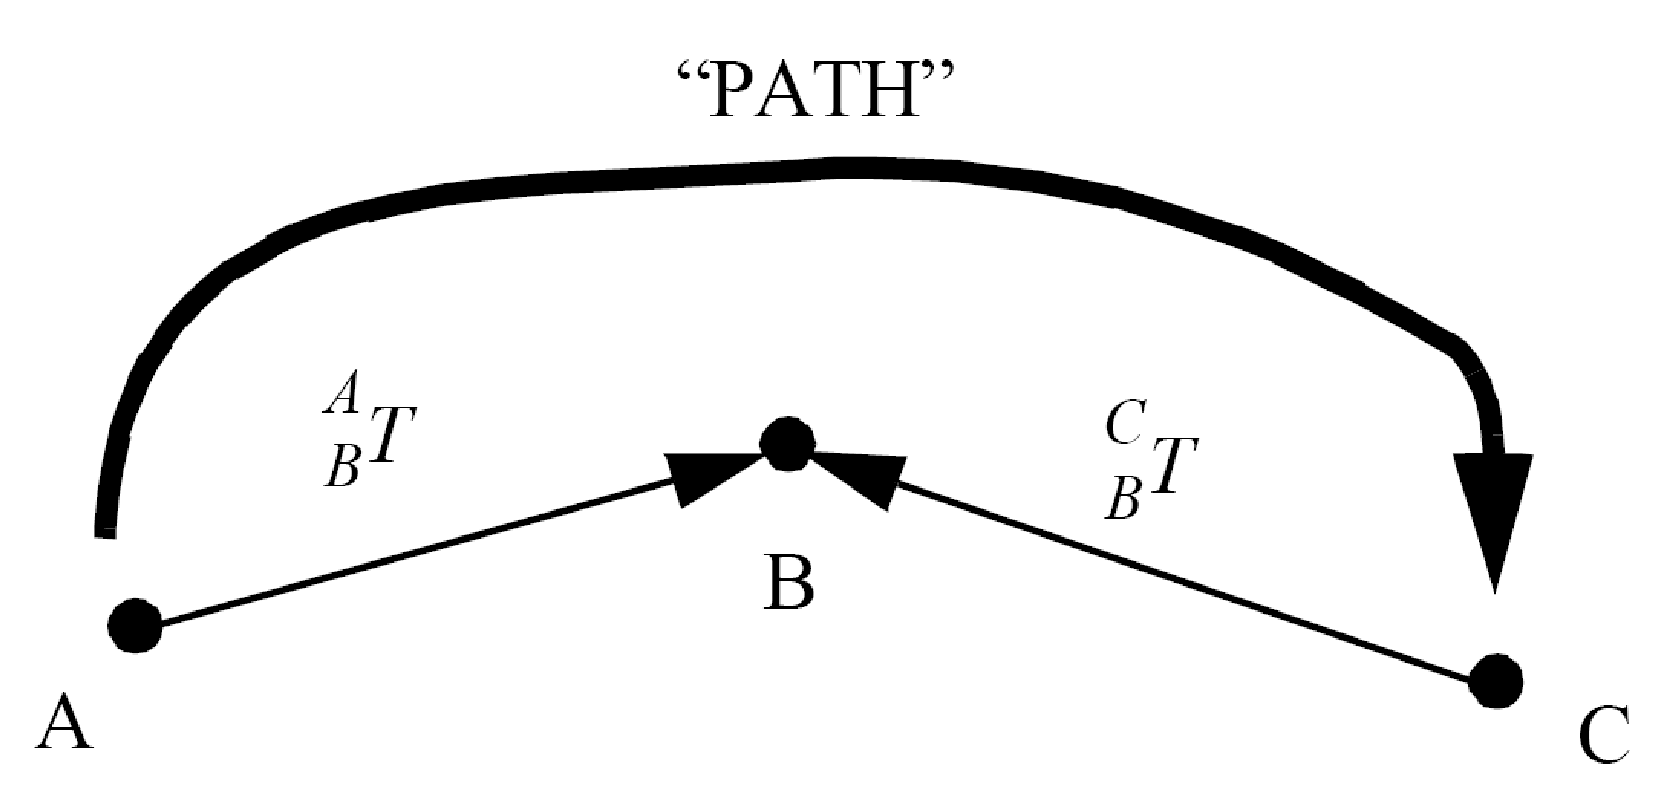
\includegraphics[width=3.5in]{figs02/abgraph.eps}
\caption{A path is  a directed arrow along a chain of transformations.}\label{PATH}
\end{figure}

The transform which shows the PATH in Figure \ref{PATH} is therefore:
\[
^A_CT = \quad ^A_BT(^C_BT)^{-1} = \quad ^A_BT^B_CT
\]
In the first right hand side, $^C_BT$ is inverted because it represents an arrow which goes opposite to the  path.
A closed path in such a graph can be cut at two nodes to form a tranform equation.

%%%%** Figure 9
\begin{figure}[h]\centering
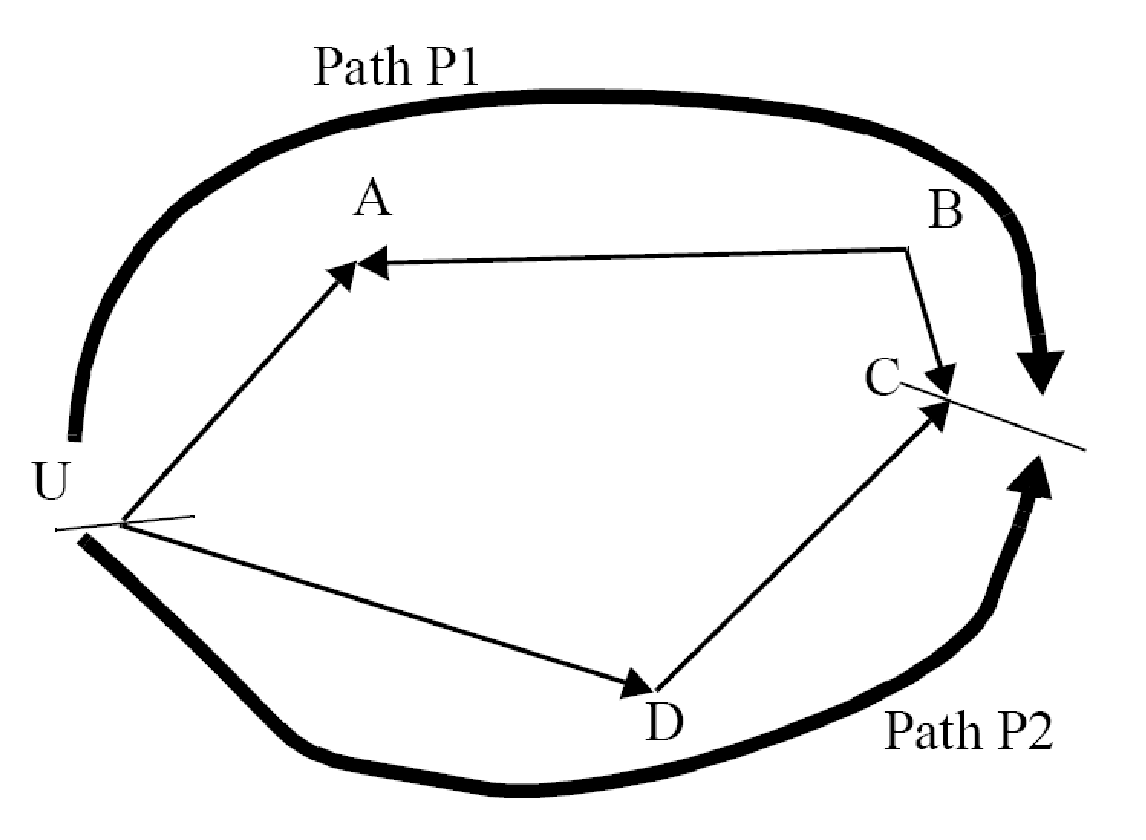
\includegraphics[width=3.5in]{figs02/xformgraph.eps}
\caption{Two paths which start and end at the same point define an equation.}\label{PATHequation}
\end{figure}

In Figure \ref{PATHequation}, the loop is cut at nodes U and C, and the two paths, P1, and P2 represent
the same displacement. Each path corresponds to an equation

\[
\mathrm{P1:} \quad  ^U_CT = ^U_AT \; ^B_AT^{-1} \; ^B_CT
\]
\[
\mathrm{P2:} \quad  ^U_CT = ^U_DT \;^D_CT
\]
And, we can equate the two right hand sides:
\[
^U_AT \;^B_AT^{-1} \; ^B_CT =  ^U_DT \;^D_CT
\]
Furthermore, we can write the equation for a big path going completely
around the loop in, for example, the clockwise direction:
\[
P1(P2)^{-1} = ^U_CT \;^U_CT^{-1} = I_{4\times4}
\]
This is expected since by going completely around the loop we wind up in our original configuration or frame.    Note that when we interpret it as a homogeneous transform, $I_{4\times4}$ corresponds to
\[
\mathrm{Rot}(x,0), \mathrm{Trans}
   \left(  \left [
    \begin{array}{c} 0 \\ 0 \\ 0  \end{array}
    \right ]  \right )
\]



\begin{Example}

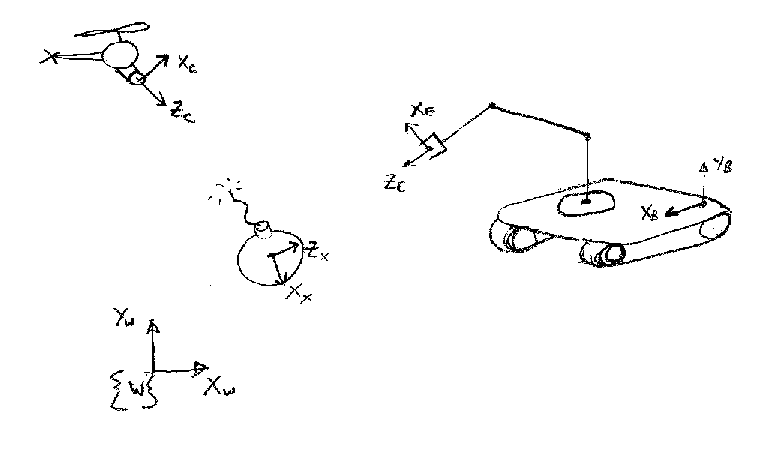
\includegraphics[width=4.75in]{figs02/00487.eps}

A helicopter mounted camera identifies the location and orientation of a bomb.  A bomb disposal robot must understand how to move its arm to pick up the bomb.  The following transforms are known:  ${^C_WT},{^C_XT},{^B_CT},{^B_ET}$

A) Draw the transform graph

B) Solve for ${^X_BT}$

C) Solve for ${^W_ET}$

Answer:

A)

\includegraphics[width=90mm]{figs02/00579.eps}

B)
\[
{^X_BT} = (^C_XT)^{-1}(^B_CT)^{-1}
\]

C)
\[
{^W_ET} = (^C_WT)^{-1}(^B_CT)^{-1}{^B_ET}
\]
\end{Example}


%%%%%%%%%%%%%%%%%%%%%%%%%%%%%%%%%%%%%%%%%%%%%%%%%%%%%%%%%%%%%%%%%%%%%%%%%%%%%%%%%%%%%%%%%%%%%%%%%%%%%%%%%%%%%%%
%
%
\begin{Example}

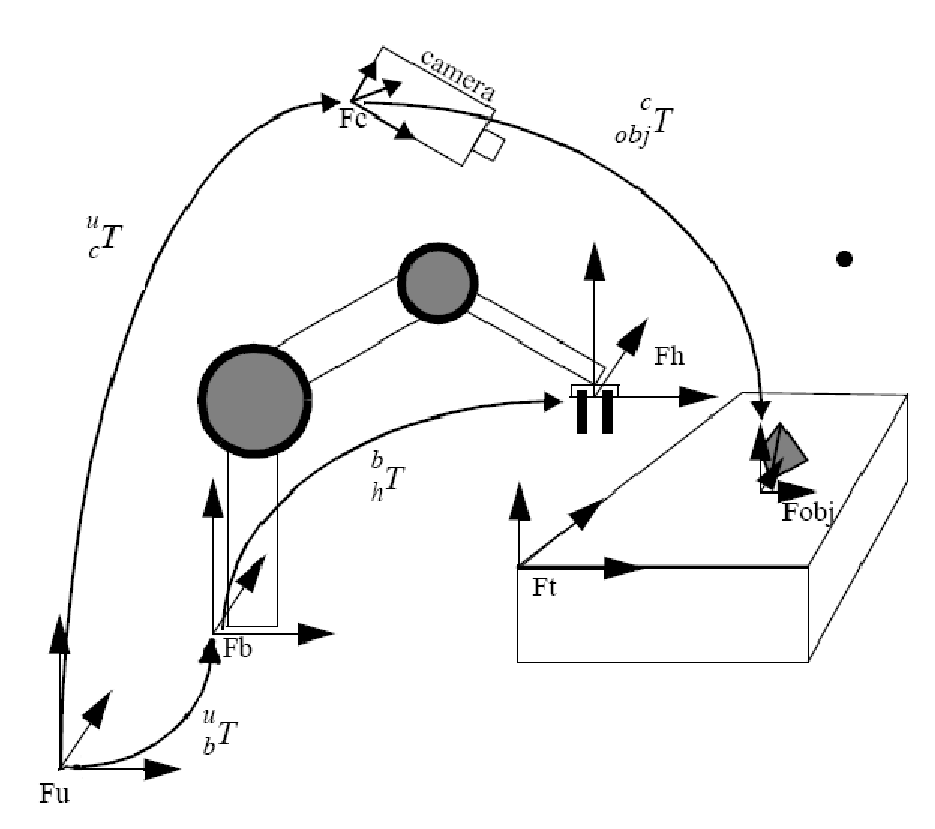
\includegraphics[width=3.5in]{figs02/camtablearmexample.eps}

Let’s consider a factory workstation with a robot arm, worktable, vision
camera, and an object on the table. The known spatial relationships are shown by links in the diagram. Suppose we need to specify the position and orientation of the object so that the robot can pick it up. The robot controller must have the configuration in Fb, the base frame of the robot.

Q1:
What is the configuration of the object in Fb?

A1:
The object can be ``reached" by a path in the transform graph from
Fb through Fu, and Fc, to Fobj. Note that the first link has a direction
opposite to the path we take to the object. The equation of this path
is:
\[
^b_{obj}T = ^u_bT^{-1} \;^u_cT \;^c_{obj}T
\]

Q2:
Suppose we want to find the unknown transforms $^h_tT, ^t_{obj}T$?

A2:
If we add these two transforms to the graph (draw them in yourself),
we now have a loop. We can cut this loop at any two points to make
an equation. Suppose we make these cuts at the hand and at the object.
Now we have
\[
^b_hT^{-1} \;^u_bT^{-1} \;^u_cT \;^c_{obj}T = ^h_tT \;^t_{obj}T
\]
Since the two transforms on the right hand side are unknown, we
cannot solve this without another equation. Now suppose we go out
to the factory floor and measure the location and orientation of the
table. This gives us $^u_tT$. Drawing this link into the transform graph, we see that another loop is formed tangent to the original loop so that we have another equation. One such equation is
\[
^u_bT \;^b_hT \;^h_tT = ^u_tT
\]
We can solve this for one of our unknowns giving:
\[
^h_tT = ^b_hT^{-1} \;^u_bT^{-1} \;^u_tT
\]
Then we substitute to get
\[
 ^b_hT^{-1} \;^u_bT^{-1} \;^u_cT \; ^c_{obj}T = ^b_hT^{-1} \;^u_bT^{-1} \;^u_tT \;^t_{obj}T
\]
\[
^c_{obj}T = ^u_cT^{-1} \;^u_tT \;^t_{obj}T
\]
\end{Example}

\begin{Example}
A revitalized GM plant has installed massive assembly robots.  Such a robot arm must install the engine into a car body.   Frames have been applied to the body and engine as shown below.

\includegraphics[width=5.5in]{figs02/00439.eps}

The following facts are known:

\begin{enumerate}
	\item The engine must be lowered through an intermediate position in order for the transmission to clear the body. This position is $^M_IT$.  Then the engine will be moved into its final position, $^M_CT$.

	\item The car and engine rack are located at known tranforms $^U_CT$, and $^U_RT$ respectively.

	\item GM has finally switched over to the metric system!
\end{enumerate}
Questions:

{\bf Q1)} Give the transform (in numerical form) which specfies the engine position in the rack, $^R_ET$.  Assume that the $z$ position coordinate is zero.

\end{Example}
\begin{ExampleCont}
\subsection*{Solution}

Obtain the rotation matrix by writing the unit vectors of {$E$} expressed in {$R$}, $or$ evaluating Rot($\hat{z},-90^{\circ}$).
\[
{^R_ET} =
\begin{bmatrix}
0 & 1 & 0 & 0.25	\\
-1 & 0 & 0 & 0.25	\\
0 & 0 & 1 & 0		\\
0 & 0 & 0 & 1
\end{bmatrix}
\]

{\bf Q2)} You need to program the robot to take the engine from the rack and put it in the intermediate position.  Solve for the transform which represents the intermediate engine position and orientation relative the engine rack, $^R_IT$ in terms of the known transforms above.

\subsection*{Solution}
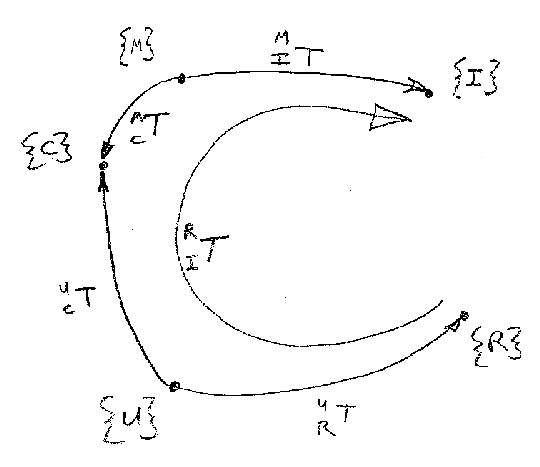
\includegraphics[width=3.5in]{figs02/00440.eps}

going around the transform graph in the direction shown, we have:
\[
{^R_IT} \quad = \quad {^U_RT^{-1}} \quad {^U_CT} \quad {^M_CT^{-1}} \quad {^M_IT}
\]
\end{ExampleCont}



\begin{Example}
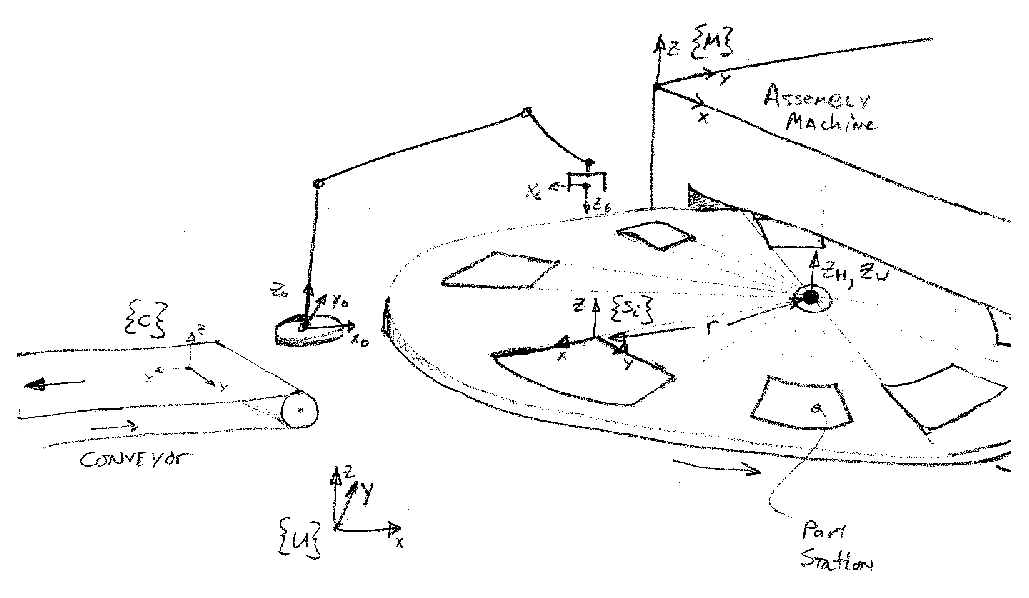
\includegraphics[width=6.4in]{figs02/00080.eps}


\subsection*{Pizza Problem}
Completed assemblies (pizzas?) come out of a machine on a large rotary
table. You must program a robot arm to pick up the pizzas and transfer
them to a conveyer.


Use the following facts:

\begin{itemize}
	\item The part stations are spaced every $36^\circ$ on the wheel.

	\item The robot base frame is \{$0$\} and the end effector frame
is \{$6$\}.

	\item The origin of frame $H$ is located at the wheel hub:
\[
^U_HT =  \left[ \begin{array}{cccc}
1 & 0 & 0 & 10  \\
0 & 1 & 0 & 10 \\
0 & 0 & 1 & 2 \\
0 & 0 & 0 & 1
\end{array}  \right]
\]
	\item The $i^{th}$ part station has frame \{$S_i$\} located at its corner.
	The distance from the origin of \{$H$\} to the origin of \{$S_i$\}
	is $r=5$.
	\item Another frame \{$W$\} has the same origin as \{$H$\}, but $X_W$
always points to the origin of \{$S_1$\}.

	\item The front panel of the machine is at
\[
^U_MT =  \left[ \begin{array}{cccc}
0  & 1 & 0 & 10  \\
-1 & 0  &0  & 16 \\
0 & 0 & 1 & 4 \\
0 & 0 & 0 & 1
\end{array}  \right]
\]

	\item $\Theta_W(t)$ describes the rotation of the wheel.  $\Theta_W$ is
the angle from $X_H$ to $X_W$.

\end{itemize}



\end{Example}


\begin{ExampleCont}
{\bf Q1:}
If $t$ is in seconds, $\Theta_W(t) =  \frac{\pi}{15}t$ rad or
$\Theta_W(t) =  12t$ degrees, what is $^U_ST(i,t)$, i.e. what is the
transform from frame $U$ to frame $S_i$ (multiply out your answer).

\subsection*{Solution:}

\[
{^U_{Si}T} \quad= \quad {^U_HT} \quad {^H_WT} \quad {^W_{Si}T}
\]
From the facts,
\[
{^H_WT} = \mathrm{Rot}(\hat{z}, 12t^{\circ})
\]
\[
{^W_{Si}T} =  \mathrm{Rot}(\hat{z}, (36(i-1))^{\circ} )
\]
\[
{^U_{H}T} \quad= \quad
\begin{bmatrix}
1 & 0 & 0 & 10	\\
0 & 1 & 0 & 10 	\\
0 & 0 & 1 &  2  \\
0 & 0 & 0 &  1
\end{bmatrix}
\]
Since the last two are both about the $\hat{z}$ axis, we can add their displacements to simplify.  Let
\[
\alpha = (12t + 36(i-1))^{\circ}
\]
Then
\[
{^U_{Si}T} \quad= \quad
\begin{bmatrix}
1 & 0 & 0 & 10	\\
0 & 1 & 0 & 10 	\\
0 & 0 & 1 &  2  \\
0 & 0 & 0 &  1
\end{bmatrix}
\mathrm{Rot}(\hat{z}, \alpha)
\]
\[
{^U_{Si}T} \quad= \quad
\begin{bmatrix}
1 & 0 & 0 & 10	\\
0 & 1 & 0 & 10 	\\
0 & 0 & 1 &  2  \\
0 & 0 & 0 &  1
\end{bmatrix}
\begin{bmatrix}
c\alpha & -s\alpha & 0 & 0	\\
s\alpha &  c\alpha & 0 & 0 	\\
0 & 0 & 1 &  0  \\
0 & 0 & 0 &  1
\end{bmatrix}
\]
\[
{^U_{Si}T} \quad= \quad
\begin{bmatrix}
c\alpha & -s\alpha & 0 & 10	\\
s\alpha &  c\alpha & 0 & 10 	\\
0 & 0 & 1 &  2  \\
0 & 0 & 0 &  1
\end{bmatrix}
\]

{\bf Q2:}
If $^U_0T, \quad ^0_6T, \quad ^U_ST(i,t)$ are known, draw a transform graph, and solve
for $^6_ST(i,t)$.

\subsection*{Solution:}

Transform Graph:

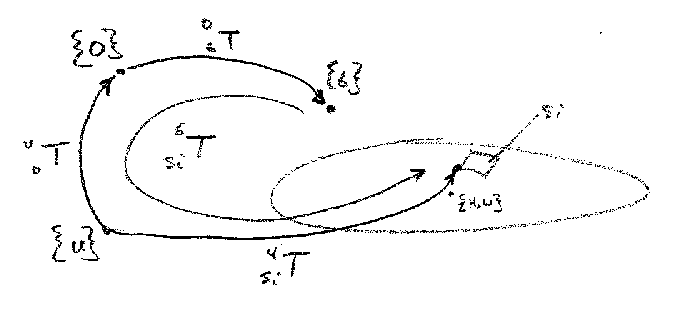
\includegraphics[width=4.3in]{figs02/00443.eps}

\[
{^6_{Si}T} \quad = \quad {^0_6T}^{-1} \quad {^U_0T}^{-1}  \quad {^U_{Si}T}
\]

\end{ExampleCont}















%
%
%
%
% \section{Quaternions}
%
% (to be written)

%  Table row height
\renewcommand\arraystretch{0.2}% Vertical Row size, 1.0 is for standard spacing)


%%%%** Section 11
\section{Exponential Coordinates}

The following elegant notation and derivation is based closely on {\bf Murray, Li, and Sastry, ``A Mathematical Introduction to Robotic Manipulation", CRC Press, 1994.}

%%%%** Section 11.1
\subsection{Rotation}\label{Rotation}

Consider the velocity of a point $q$ which is rotating about an axiz $\omega$.  We assume that
$|\omega|=1$ and its direction is the axis of rotation. We can write the velocity of the point as
\[
\dot{q}(t)=\omega \times q(t)
\]

Recall that the vector cross product ($\times$) can be represented as the product of a special
skew-symmetric matrix,
\[
\hat{\omega} = \left[
\begin{array}{ccc}
0               &       -\omega_3       &       \omega_2      \\
\omega_3        &       0               &       -\omega_1     \\
-\omega_2       &       \omega_1        &       0             \\
\end{array}
\right]
\]
with the vector, i.e.
\[
\omega \times q = \hat{\omega} q
\]
So we have
\[
\dot{q}(t)=\hat{\omega} q(t)
\]
This is a first order differential equation with the solution
\[
q(t) = e^{\hat{\omega}t}q(0)
\]

Now we need to understand what it means to take the exponential of a matrix!
Using the Taylor series expansion, we have:
\[
\exp(A) = I + A + \frac{A^2}{2!} + \frac{A^3}{3!} + ...
\]
We are interested in the special case of
\[
A = \hat{\omega}t
\]
where $\hat{\omega}$ is the matrix defined as above and $t$ is a scalar (time).
One interpretation is that we can parameterize any rotation by the amount of time
it takes at unit velocity ($|\omega|=1$). Thus we can also write
\[
R(\omega,\Theta) = e^{\hat{\omega}\Theta}
\]
where
\[
\Theta = |\omega|t
\]

To evaluate the matrix exponential, we sort the series out into odd and even terms (and perform
a few other tricks) to get:
\[
e^{\hat{\omega}\Theta} =
    I
 +
    \left(
       \Theta - \frac{\Theta^3}{3!} + \frac{\Theta^5}{5!} + \dots
    \right)\hat{\omega}
 +
    \left(
       \frac{\Theta^2}{2!} + \frac{\Theta^4}{4!} + \frac{\Theta^6}{6!} + \dots
    \right)\hat{\omega}^2
\]
Which simplifies to
\[
e^{\hat{\omega}\Theta} = I + \hat{\omega} \sin \Theta + \hat{\omega}^2(1-\cos\Theta)
\]
So $e^{\hat{\omega}\theta}$ is the rotation matrix which expresses rotation by $\theta$ about
axis $\omega$.

This can also be inverted (See Murray, Li, Sastry, equations (2.17) and (2.18),
or Craig, equations (2.81) and (2.82)):
\begin{equation}\label{thetainverse}
\theta = cos^{-1} \left(
        \frac {r_{11} + r_{22} + r_{33} -1}
              {2}
        \right)
\end{equation}
\begin{equation}\label{omegainverse}
\omega = \frac{1}{2sin\theta} \left[
        \begin{array}{c}
        r_{32}-r_{23}   \\
        r_{13}-r_{31}   \\
        r_{21}-r_{12}   \\
        \end{array}
        \right]
\end{equation}




%%%%** Section 11.2
\subsection{Translation and Rotation}
Consider a point, $p(t)$ whos position is a function of time.  Assume that the point is displaced due to
rotation about an axis, $\omega$, separate from the point.  We assume that $|\omega|=1$ and that $q$ is
a point {\bf off} the axis. The velocity of the point is then
\[
\dot{p}(t) = \omega \times (p(t) - q)
\]
or
\[
\dot{p}(t) = \omega \times p(t) - \omega \times q
\]
Using $\hat{\omega}$ as defined above, if we define
\[
\hat{\xi} = \left[
\begin{array}{cc}
\hat{\omega}   &       -\omega\times q \\
0       &       0       \\
\end{array}
\right]
\]
and we express $p(t)$ and its derivative in homogeneous coordinates,
\[
\dot{p} =  \left[
\begin{array}{cc}
\hat{\omega}   &       -\omega\times q \\
0       &       0       \\
\end{array}
\right]
\left[
\begin{array}{c}
p\\
1\\
\end{array}\right]
\]
In this special case (of rotation about an axis remote from $\omega$) the velocity
of the point $p$ is $-\omega\times q$.  More generally, we can write
\[
\dot{p} =  \left[
\begin{array}{cc}
\hat{\omega}   &       v \\
0       &       0       \\
\end{array}
\right]
\left[
\begin{array}{c}
p\\
1\\
\end{array}\right]
\]

More compactly:
\[
\dot{p} = \hat{\xi}p
\]

the matrix $\hat{\xi}$ is refered to as a {\it twist}.

This is a first order differential equation which has the solution:
\[
p(t) = e^{\hat{\xi}t}p(0).
\]
Recall that $\hat{\xi}$ doesn't have as simple a form as $\hat{\omega}$ and so it is
not as easy to get an expression for $e^{\hat{\xi}t}$.
It can be shown that (see Murray, Li, and Sastry, Proposition 2.8) that for a displacement which
consists of rotation $\hat{\omega}\Theta$ and displacement $v\theta$
\begin{equation}\label{matrixexp}
e^{\hat{\xi}\theta} =
\left[
  \begin{array}{cc}
  e^{\hat{\omega}\theta}   & (I-e^{\hat{\omega}\theta})(\omega\times v) + \omega\omega^Tv\theta          \\
  0                        &       1                               \\
  \end{array}
\right]
\end{equation}

As used here, $\theta$ is a general motion parameter and need not be an angle.
The interpretation of $e^{\hat{\xi}\theta}$ is a description of a physical manipulation
i.e.
\[
^Ap(\theta) = {e^{\hat{\xi}\theta}}    {^Ap(0)}
\]
Note that both $^Ap(\theta)$ and $^Ap(0)$ are represented in the same frame, $A$, which
should also be the same as that used for $\omega$ and $v$.

To represent a known physical displacement as a twist, we first must know the 4x4 homogeneous
transform defining the displacement, $^A_BT$ which the authors call $g_{ab}$.
Given $g_{ab}$, we solve for the ``twist coordinates", $\omega, \theta, v$ equating
(\ref{matrixexp}) with the known $g$:
\[
g = \left [
        \begin{array}{cc}
        R               &               P       \\
        0               &               1       \\
        \end{array}
\right]
=
\left[
        \begin{array}{cc}
  e^{\hat{\omega}\theta}   & (I-e^{\hat{\omega}\theta})(\omega\times v) + \omega\omega^Tv\theta          \\
  0                        &       1                               \\
        \end{array}
\right]
\]
for
\[
R = e^{\hat{\omega}\theta}
\]
we had equation (\ref{thetainverse} and (\ref{omegainverse}) to find $\theta$ and $\omega$.
To get $v$, we have
\[
P = (I-e^{\hat{\omega}\theta})(\omega\times v) + \omega\omega^Tv\theta
\]
which we can solve by hand calculation or Mathematica for $v$.  There are some useful special
cases. For example for a simple axis such as
\[
\omega = \left [
        \begin{array}{c}
        0\\0\\1\\
        \end{array}
        \right ]
\]
the equation to solve is
\[
\left[
        \begin{array}{ccc}
        s\theta &       c\theta -1      &       0\\
        1-c\theta   &   s\theta         &       0\\
        0              &        0       &   \theta\\
        \end{array}
\right]
v = P
\]
In the special case of revolute motion about the axis $\omega$, $v$ is only due to the
rotation and so it is known:
\[
v = -\omega \times q
\]

%%%%** Section 11.3
\subsection{Groups}
Murray, Li, and Sastry take some pains to relate these kinematic ideas to group theory.
The basic properties of a group are
\begin{itemize}
        \item It consists of a set of objects, $G$ and a binary operation, $\times$.
        \item It is ``closed" in the sense that if any two objects in the
        group are applied to the binary operation, the result is another member
        of the group.
        \item There exists an ``identity element", $i$, which is a member of the
        group such that $g \times i = g$.
        \item For every element of the group, $g$, there is a unique inverse, also a
        an element of the group, $g^{-1}$
         such that $g\times g^{-1} = i$.
        \item The operation is associative:  $(g_1\times g_2)\times g_3= g_1 \times (g_2\times g_3)$.
\end{itemize}
For example, you can verify that these five properties hold for the set of orthonormal 3x3 rotation matrices together with
the operation of matrix multiplication, and so they must form a group.

Murray, Li, and Sastry named four groups which are relevant to robotic manipulation:
\begin{description}
        \item[$se(3)$] the group of 4x4 skew symmetric matrices (twists)
        \item[$so(3)$] the group of 3x3 skew symmetric matrices ($\hat{\omega}$).
        \item[$SE(3)$] the group of 4x4 homogeneous transforms
        \item[$SO(3)$] the group of 3x3 orthonormal rotation matrices
\end{description}


%%%%** Section 12
\section{Summary of Notation}

% Summary of Notation for Chapter  02

